\subsection{Extra data by-product}

As mentioned before, after the data is ingested into BigQuery, our team will try to extract some
value and insight from the data itself. This will include: a product recommendation and a sale
visualizing dashboard.

\subsubsection{Personal Product Ranking}

\subsubsection{Sale visualizing dashboard}
BigQuery supports a built-in tool, called Data Canvas, that help Data Scientists and Data Analytics
to quickly perform visualization and aggregation, without the need for an external tool.

With the objective of building a dashboard, to visualize the total sale's net value Day-over-day, we
first created a new Data canvas in BigQuery. Then, we build the query to sum all the sale net
values, group by invoice date. BigQuery is great here, as it provides a prompt to help ease the
process of experimenting with data. We can also see a preview of the data in the bottom pane.

When we are happy with the query, our team select \textbf{Visualization} to invoke BigQuery drawing
graphs based on the above query.

\begin{figure}[htp]
    \centering
    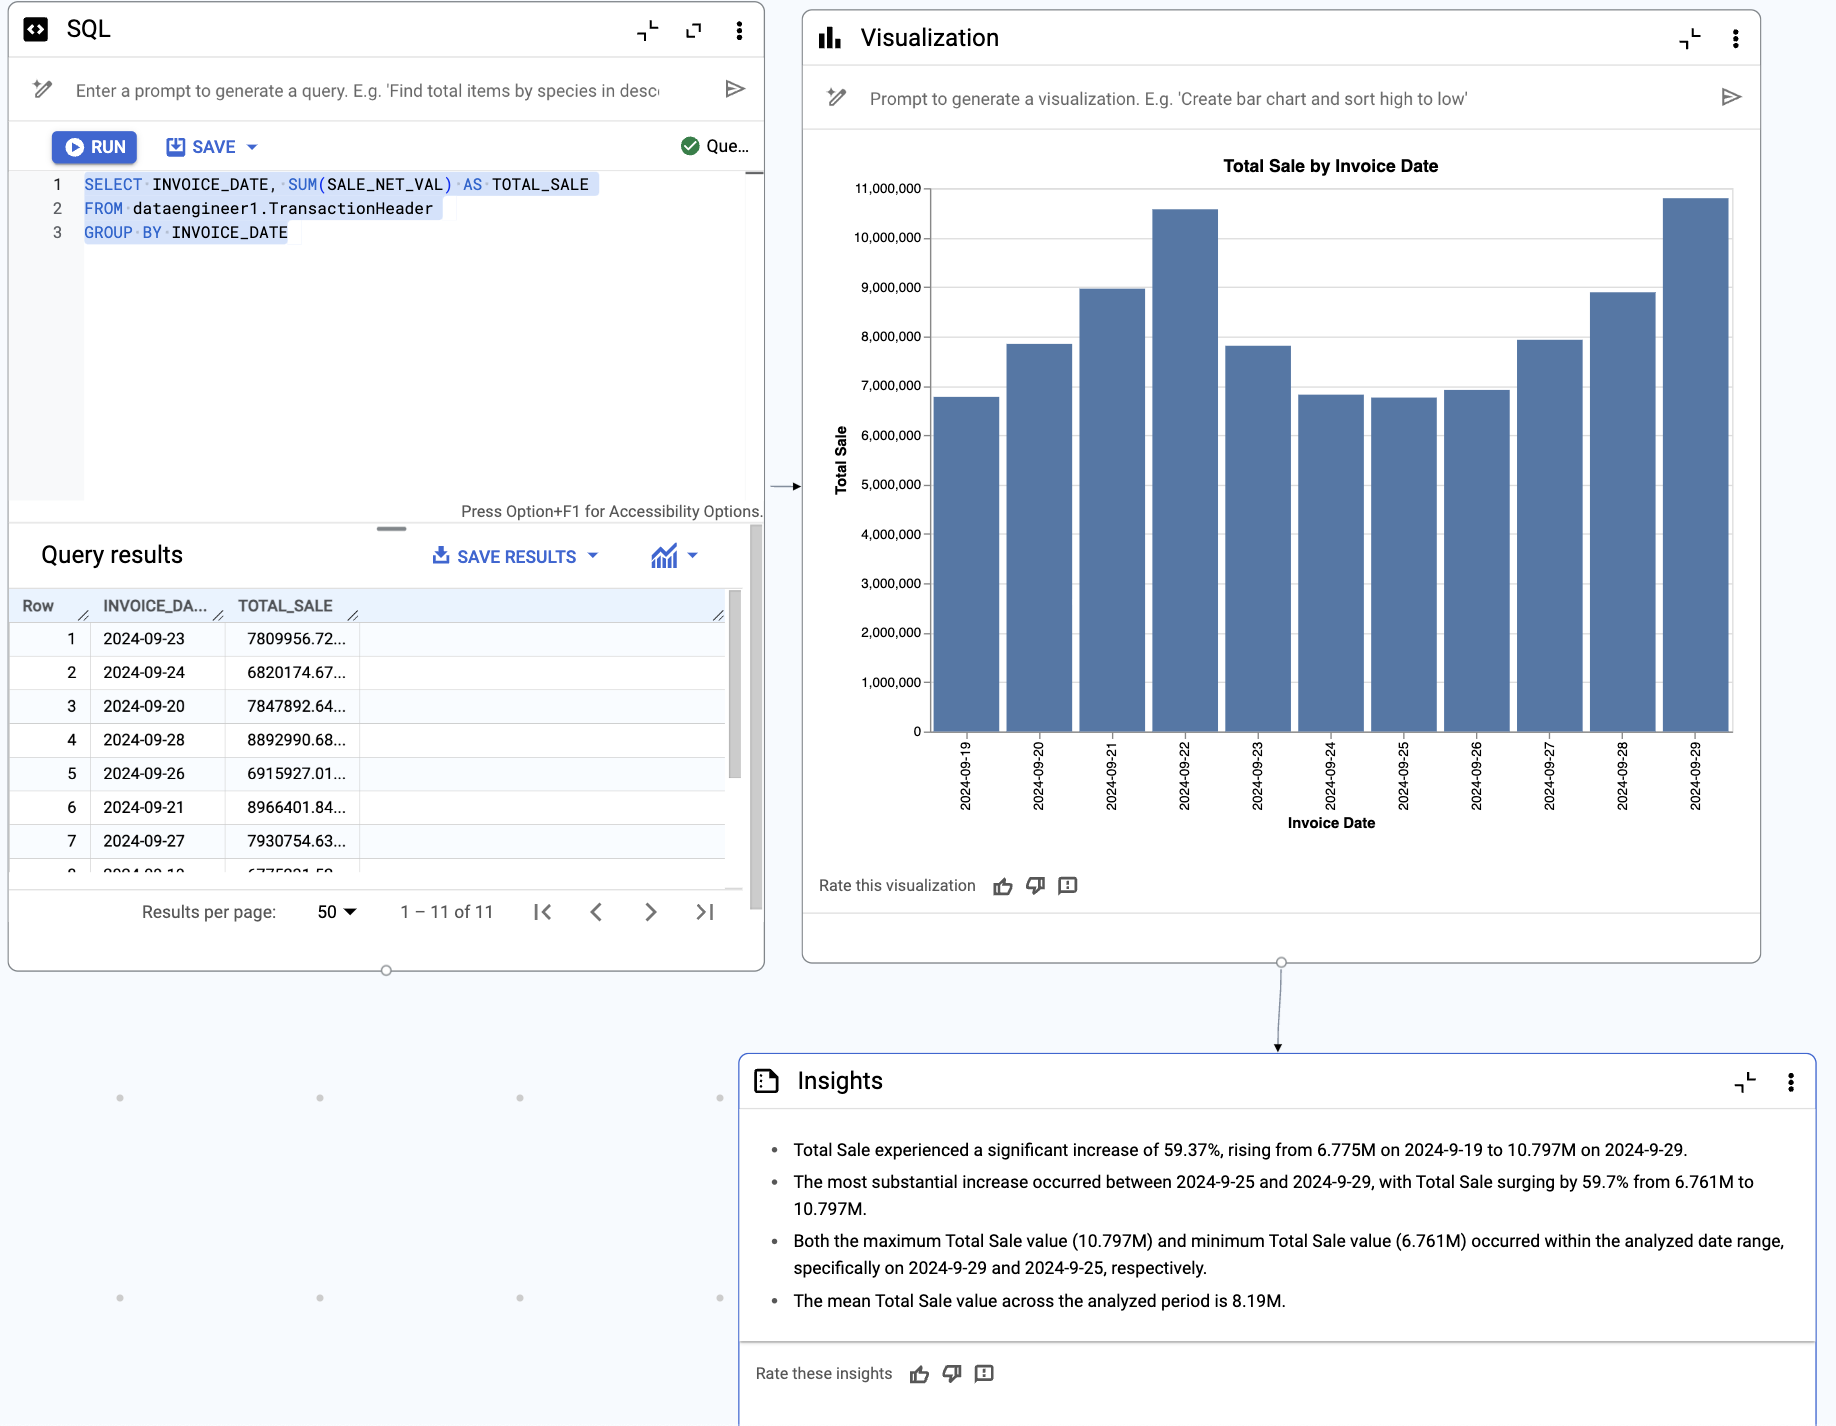
\includegraphics[width=\linewidth]{images/data_canvas.png}
    \caption{Visualizing sales within data period}
\end{figure}

\subsubsection{Data Insights}
BigQuery also supports a feature for generating insights from the provided data. We find this tools
really interesting, in that it helps quickly summarize data without manual typing.

Combining with those generated-insights, here are what our team has found about the sales:
\begin{enumerate}
    \item Total Sales experienced a remarkable increase of 59.37\% over the analyzed period, rising
    from 6.775 million on September 19, 2024, to 10.797 million on September 29, 2024. This notable
    growth reflects a dynamic upward trend in the sales data.
    \item The most significant growth occurred toward the end of the period, between September 25
    and September 29, 2024. During this time, Total Sales surged by 59.7\%, jumping from 6.761
    million to 10.797 million, marking the steepest increase within the analyzed timeframe.
    \item The dataset's maximum and minimum Total Sales values were both recorded during this
    period, highlighting its dynamic nature. The highest value, 10.797 million, was observed on
    September 29, 2024, while the lowest value, 6.761 million, occurred on September 25, 2024.
    \item On average, Total Sales during the analyzed period amounted to 8.19 million. This mean
    value underscores the overall growth trajectory while accounting for fluctuations within the
    observed dates.
    \item During a week, sales is usually at its highest in the weekend (Saturday and Sunday). It
    also decrease significantly between Monday and Wednesday, when the steepness slow down.
\end{enumerate}